\section{Methods}
\par Shughni has multiple dictionary options, as we learned in the previous section. My choice fell for the dictionary made by \textcite{karamshoev_dict_1988} since it is the latest and the biggest dictionary. And moreover, researchers from the `Digital Resources for the Shughni Language' project \parencite{makarov_digital_2022} created an online Karamshoev's dictionary of the Shughni language. They granted me access to the underlying database from where it is easily possible to export all the needed lexemes and their meta information like POS tags or verb's tense and aspect.
\par Regarding the choice of the grammatical description, as the main source I have selected the one provided by \textcite{parker_shughni_2023} as the most suitable foundation for this study. This work offers an exceptionally thorough analysis of Shughni morphology including a very detailed inflectional paradigm description. In addition, I also will be using the inside materials of the 2019 -- 2024 HSE expeditions to Tajikistan.
\par The morphological parser will be developed using Helsinki Finite-State Technology (HFST) \parencite{linden_hfst_2009}, which is a tool set for working with rule-based morphology models in a form of transducers. Finite-state transducer (FST) is a finite-state machine that works with two tapes, following the terminology for Turing machines \parencite{Turing_1937}: it reads strings of text from the input tape and writes strings of text to the output tape. When FST receives an input string, it walks along its characters from one state to another as long as there is a valid transition from the current state with an upcoming letter, see Figure \ref{fig:fst1} for visualization. It stops when it reaches an end state (marked as a double-lined circle on the Figure \ref{fig:fst1}) and then the output tape's string is considered to be a valid output. If there is no valid path to an end state then the output tape's string is discarded. There are usually multiple end states present, not just one, as on the Figure \ref{fig:fst1}.
\begin{figure}[!ht]
    \centering
    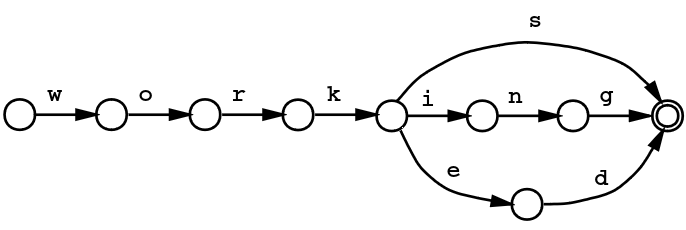
\includegraphics[scale=0.5]{\rootdir/img/transducer1.png}
    \caption{An example of FST for a language where only three words exist: \textit{works}, \textit{working} and \textit{worked}. The word \textit{worker}, for example will not be recognized as a valid word by this FST, since there is no 'd' transition at state \textit{worke}. The only way from \textit{worke} state is via 'd' transition, which corresponds to the \textit{worked} word. \parencite{beesley_fst_2002}}
    \label{fig:fst1}
\end{figure}
\par As FST walks through states (on Fig.\ref{fig:fst1} states are graph's nodes) on each transition (on Fig.\ref{fig:fst1} transitions are graph's edges) it can read an input tape and/or write to the output tape. A syntax for transitions is \textit{`x:y'}, which means `read \textit{x} from input, write \textit{y} to output'. Transition will happen only if input matches. With this in mind we can turn FST from Figure \ref{fig:fst1} into a morphological analyser by modifying some transitions (See Fig. \ref{fig:fst1_1}). Syntax \textit{`x:'} means that FST must write nothing to the output tape while still making a transition to the next state if input matches.
\begin{figure}[!ht]
    \centering
    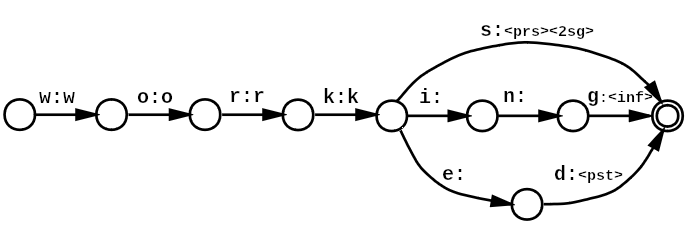
\includegraphics[scale=0.5]{\rootdir/img/transducer1_1.png}
    \caption{A modified version of Figure \ref{fig:fst1} which takes as input \textit{works}, \textit{working}, \textit{worked} and outputs \textit{work<prs><2sg>}, \textit{work<inf>}, \textit{work<pst>} respectively.}
    \label{fig:fst1_1}
\end{figure}
\par HFST is a modern tool set, it allows working with a wide range of compilers in a single shared FST format. Instead of built-in \texttt{hfst-lexc} I will be using \texttt{lexd} compiler. Even thought it is not included into the HFST, it still produces transducers in HFST format. The choice between \texttt{lexc} and \texttt{lexd} was made in the latter's favor since it is a newer, more optimized and faster version of \texttt{lexc}. The other option is Xerox's \texttt{xfst} compiler, which is a quite outdated option and was rarely used outside of Xerox. The advantage of \texttt{lexc} is its tag system, which allows tagging stems and affixes, allowing to tune the combination of the lexemes with specific tags. This feature allows us to minimize overgeneration of unwanted FST paths.
\par For the matter of the morphonology part, HFST's implementation of TWOLC (\texttt{hfst-twolc}) will be used. Shughni is not rich for morphonology, but it still has some rules like the insertion of \textit{`y'} on the phoneme border between two vowels, which is not possible to model using only a lexicon compiler.
\par The quality of the product morphological parser will be measured using two metrics: \textit{coverage} and \textit{accuracy}. The \textit{coverage} is calculated as follows: \[coverage = \frac{N_{rec}}{N_{total}}\] where $N_{rec}$ is the amount of tokens, that the parser was able to recognize and return any output, and $N_{total}$ is the total amount of tokens. As of now, texts for \textit{coverage} evaluation are the Luke book of the Bible, a fairy tale and a collection of short miscellaneous texts with the total amount of 187149 tokens. All these texts were provided to me by \textcite{makarov_digital_2022}. The formula for \textit{accuracy} is: \[accuracy = \frac{N_{correct}}{N_{rec}}\] where $N_{correct}$ is the amount of tokens for which the parser gave the same set of morphological tags as a human linguist did manually and $N_{total}$ is the total amount of recognized tokens. The manually tagged texts were also provided by `Digital resources for the Shughni Language' project. The tagged texts consist of 3453 tokens in total.
\par The core of the model will be written around Cyrillic stems and affixes. Then a separate FST for transliteration will be attached to the Cyrillic FSTs to make transducers that are able to work with Latin script.
\par The format of the tagged version of token \textit{`working'} will be \textit{`work<v>{}><inf>'}. Each tag is encapsulated into angular brackets and the morpheme border will be represented by a single `greater than' or `right angular bracket' sign. The tagged token \textit{`work<v>{}><inf>'} is an equivalent of \textit{`work.V-INF'} in standard linguistic notation. The motivation for morpheme `>` separator is that it is a standard for Apertium's systems and this format may be assumed by the outside user. This decision is not final since it brings complications with parsing of this format because this separator matches morpheme border bracket.